\documentclass[10pt]{beamer}
\usepackage{kotex}

\usepackage{framed}
%https://www.overleaf.com/learn/latex/Inserting_Images


\usepackage{amsthm}
%use dfrac
\usepackage{thmtools}
\usepackage{lipsum}
\usepackage{url}
\usepackage{amsmath}
\usepackage{amssymb}
%\usepackage{ansform}
\usepackage{thmtools}
\usepackage{graphicx}
%https://www.overleaf.com/learn/latex/Inserting_Images

\usepackage{listings}
\usepackage{xcolor}
\declaretheoremstyle[% spaceabove=6pt,spacebelow=6pt, headfont=\color{MainColorOne}\sffamily\bfseries, notefont=\mdseries, notebraces={[}{]}, bodyfont=\normalfont,
headpunct={},
postheadspace=1em,
%qed=▣,
]{maintheorem}

\declaretheorem[%
name=정의,
style=maintheorem,
numberwithin=section, shaded={%bgcolor=MainColorThree!20,
margin=.5em}]{dfn}
% \begin{dfn}[]
% \end{dfn}

%\newtheorem{theorem}{Theorem}[section]
%\newtheorem{corollary}{Corollary}[theorem]
%\newtheorem{lemma}[theorem]{Lemma}
%https://www.overleaf.com/learn/latex/Theorems_and_proofs



\usepackage{amsthm}
%\usepackage{tabl}
\usepackage{listings}
\definecolor{mGreen}{rgb}{0,0.6,0}
\definecolor{mGray}{rgb}{0.5,0.5,0.5}
\definecolor{mPurple}{rgb}{0.58,0,0.82}
\definecolor{backgroundColour}{rgb}{0.95,0.95,0.92}
%https://tex.stackexchange.com/questions/348651/c-code-to-add-in-the-document
\lstdefinestyle{CStyle}{
    backgroundcolor=\color{backgroundColour},   
    commentstyle=\color{mGreen},
    keywordstyle=\color{magenta},
    numberstyle=\tiny\color{mGray},
    stringstyle=\color{mPurple},
    basicstyle=\footnotesize,
    breakatwhitespace=false,         
    breaklines=true,                 
    captionpos=b,                    
    keepspaces=true,                 
    numbers=left,                    
    numbersep=5pt,                  
    showspaces=false,                
    showstringspaces=false,
    showtabs=false,                  
    tabsize=2,
    language=C
}

\usepackage{url}

\usepackage{etoolbox}
\AtBeginEnvironment{quote}{\singlespacing\small}



\setbeamertemplate{footline}[frame number]

\usetheme{Hannover}
%\usetheme{CambridgeUS}


\title{Quick Sort}

\author{EUnS}

\begin{document}


\begin{frame}{}
    \maketitle
\end{frame}    

% \begin{frame}{}
%     \tableofcontents
% \end{frame}   


\begin{frame}[fragile]{}
    \begin{lstlisting}[style = Cstyle]
    QUICKSORT(A, p, r)
        if p < r
            q = PARTITION(A, p, r)
            QUICKSORT(A, p, q - 1)
            QUICKSORT(A, q + 1, r)
    \end{lstlisting}
    \pause
    \begin{lstlisting}[style = Cstyle]
    PARTITION(A, p, r) // Lumoto
        x =A[r]
        i = p - 1
        for j = p to r - 1
            if A[j] <= x
                i = i + 1
                exchange A[i] with A[j]
        exchange A[i + 1] with A[r]
        return i + 1
    \end{lstlisting}
\end{frame}    


\section{대략적인 복잡도 분석}

\subsection{최악의 분할 케이스} 

\begin{frame}{최악의 경우 분할 케이스}
    \pause
    \begin{itemize}
        \item 왼쪽 오른쪽 분할이 한쪽으로 쏠려(오름차순,내림차순) 극도로 불균형하게 일어났을때
        \pause
    \end{itemize}
    $$T(n) = T(n-1) + cn $$
    \pause
    \[
        \begin{aligned}
            T(n) &= T(n-1) + cn \\ \pause
            &= T(n-2) + c(n-1) +cn \\  \pause
            &= c\sum^{n}_{k=1}k \\ \pause
            &= \dfrac{1}{2} cn^{2}\\ \pause
            &= \Theta (n^{2})    
        \end{aligned}
    \]
\end{frame}


\begin{frame}{최선의 분할 케이스}
    \pause
    \begin{itemize}
        \item 정확하게 반으로 나누어 졌을때
    \end{itemize}
    \pause
    $$T(n) = 2T\left( \dfrac{n}{2}  \right) + cn $$
    \begin{itemize}
        \item 마스터 정리 case 2
    \end{itemize}
    $$\Theta(n\log n)$$
    
\end{frame}

\subsection{일반적인 케이스 직관적인 방법} 
\begin{frame}
    \begin{itemize}
        \item 항상 9:1로 분할하는 경우
        \item 최악의 경우와 최선의 경우가 번갈아 나타나는 경우
    \end{itemize}
\end{frame}

\subsubsection{항상 9:1로 분할하는 경우}

\begin{frame}{$9:1$로 분할}
    \begin{figure}[h!]
        %\centering
        \raggedleft
        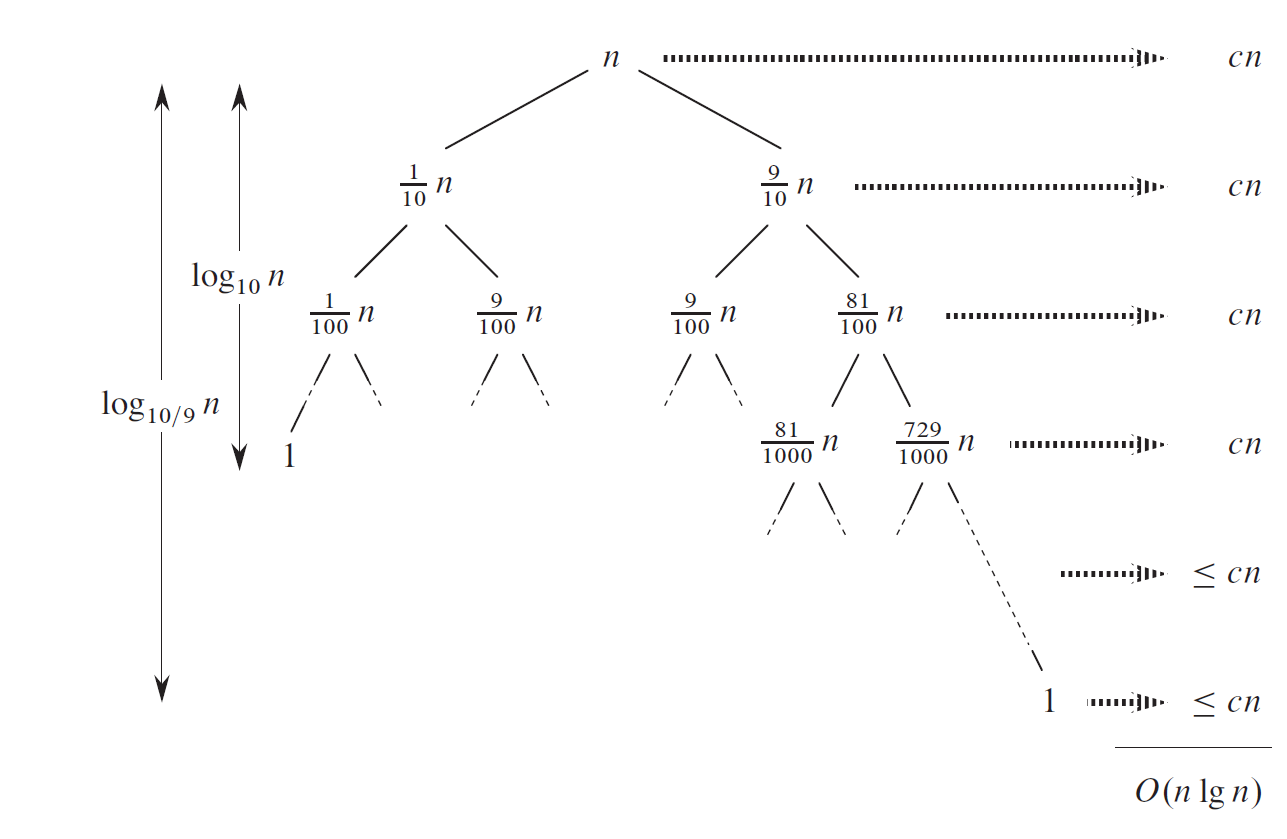
\includegraphics[scale=0.3]{./QuickSort/pic/q9.png}
        \caption{9:1로 분할하는 재귀 트리\cite{reference1}}
    \end{figure}
\end{frame}



\begin{frame}{}
    \begin{itemize}
        \item $T(n) \le T\left(\dfrac{9n}{10}\right) + T\left(\dfrac{n}{10}\right)+ cn$
        \pause
        \item $n\log_{10/9}n = O(n \log n)$
    \end{itemize}
\end{frame}

\subsubsection{최악의 경우와 최선의 경우가 번갈아 나타나는 경우}


\begin{frame}{최악 최선}
    \begin{figure}[h!]
        \centering
        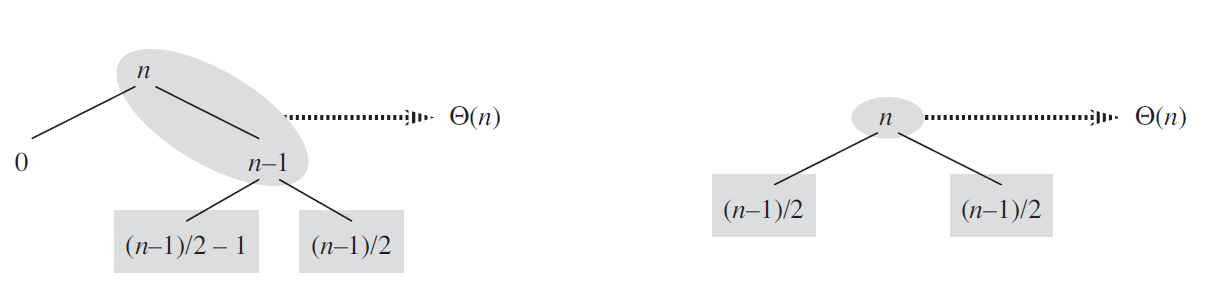
\includegraphics[scale=0.3]{./QuickSort/pic/q3.png}
        \caption{최악,최선이 번갈아 나타나는 재귀 트리\cite{reference1}}
    \end{figure}
    \pause
    \begin{itemize}
        \item $T(n)$ $T(n-1)$ 둘다 $\Theta(n)$
        \pause
        \item $\Theta(n \lg n)$
    \end{itemize}
\end{frame}


\section{상세 분석}

\subsection{최악의 케이스 분석}

\begin{frame}{최악의 케이스 분석}
    \begin{itemize}
        \pause
        \item $$T(n) = \max_{0 \le q \le n-1}(T(q) + T(n-q-1)) + \Theta(n)$$
        \pause
        \item $T(n) \le c_1n^2$이라 가정
        \pause
        \item $$T(n) \le \max_{0 \le q \le n-1}(c_1q^2 + c_1(n-q-1)^2) + \Theta(n)$$
        \pause
        \item $f(q) = c_1q^2 + c_1(n-q-1)^2 (0 \le q \le n-1)$
        \pause
        \item 극댓값이자 최댓값은 $q=0$일때와 $q=n-1$일때 둘중하나.
    \end{itemize}    
\end{frame}

\begin{frame}
    \[
        \begin{aligned}
            T(n) & \le c_1(n-1)^2 + \Theta(n) \\ \pause
            & \le c_1n^2 - c(2n-1) + \Theta(n) \\ \pause
            & \le c_1n^2    
        \end{aligned}
    \]
\end{frame}

\subsection{기대 수행 시간}

\begin{frame}{기대 수행 시간}
    \begin{lemma}
        크기가 n인 배열에 대해 QUICKSORT의 전체 실행 동안 PARTITION의 4행에서 수행되는 비교 횟수를 X라 하자. QUICKSORT의 실행시간은 O(N+X)이다.    
    \end{lemma}
    \pause
    \begin{proof}
        알고리즘은 PARTITION을 최대 n회 호출한다. 각 호출은 for 루프를 실행하는데, for 루프의 각 반복은 4행 비교문을 실행한다.    
    \end{proof}
\end{frame}


\begin{frame}{}
    \begin{itemize}
        \item 각 호출에 대한 비교를 분석하지않고 총 비교수를 계산 \pause
        \item 배열 $A = \{z_1 , z_2, ... , z_n\}$의 각 요소가 내림차순으로 정렬  \pause
        \item 집합 $Z_{ij} = \{z_i, z_{i+1}, ..., z_j\}$ 
        \pause
        \item $z_i$와 $z_j$는 최대 한번 비교
        \pause
        \item PARTITION에서 비교를 하는 경우는 하나의 원소가 pivot으로 선택 되었을 때인데, 이후에 이 pivot은 절대로 다른 원소와 비교하지 않는다.
    \end{itemize}
\end{frame}
%indicator random variables


\begin{frame}{}
    \begin{itemize}
        \item $X_{ij} = I\{ z_i$가 $z_j$와 비교한다 $\}$  \pause
        \item $ \displaystyle X = \sum_{i=1}^{n-1}\sum_{j=i+1}^{n} X_{ij}$
    \end{itemize}
    
    \[
        \begin{aligned}
            E[x] &= E \left[ \sum_{i=1}^{n-1}\sum_{j=i+1}^{n} X_{ij} \right] \\ \pause
            &= \sum_{i=1}^{n-1}\sum_{j=i+1}^{n} E\left[X_{ij} \right] \\ \pause
            &= \sum_{i=1}^{n-1}\sum_{j=i+1}^{n}Pr\{ z_i \mbox{가} z_j\mbox{와 비교한다} \} 
        \end{aligned}    
    \]
\end{frame}


\begin{frame}

\[
    \begin{aligned}
        Pr\{ z_i \mbox{가} z_j\mbox{와 비교한다}\} \\ \pause
        = Pr\{ Z_{ij}\mbox{에서} z_i \mbox{또는} z_j\mbox{가 첫번째로 선택된다.}\} \\ \pause
        = Pr\{ Z_{ij} \mbox{에서} z_i \mbox{가 첫번째로 선택된다}.\} \\ \pause
        + Pr\{ Z_{ij}\mbox{에서} z_j \mbox{가 첫번째로 선택된다.}\} \\ \pause
        = \dfrac{1}{j-i+1} + \dfrac{1}{j-i+1} \\ \pause
        = \dfrac{2}{j-i+1}    
    \end{aligned}
\]


\end{frame}

    
\begin{frame}{상한}
    
$$E[X] =  \sum_{i=1}^{n-1}\sum_{j=i+1}^{n} \dfrac{2}{j-i+1}$$  \pause
$j-i$을 $k$로 치환  \pause

\[
    \begin{aligned}
        E[X] & = \sum_{i=1}^{n-1}\sum_{j=i+1}^{n} \dfrac{2}{j-i+1}\\ \pause
        & =  \sum_{i=1}^{n-1}\sum_{k = 1}^{n-i} \dfrac{2}{k+1} \\ \pause
        & \le \sum_{i=1}^{n-1}\sum_{k = 1}^{n} \dfrac{2}{k} \\ \pause
        & \le \sum_{i=1}^{n-1} c\lg n \\ \pause
        & \le c n \lg n    
    \end{aligned}
\]
\end{frame}

\begin{frame}{}
    \[
        \begin{aligned}    
        E[X] &= \sum_{i=1}^{n-1}\sum_{k = 1}^{n-i} \dfrac{2}{k+1} \\ \pause
        & = \sum_{k = 1}^{n-1} \dfrac{2}{k+1} + \sum_{k = 1}^{n-2} \dfrac{2}{k+1} + \cdots + \sum_{k = 1}^{1} \dfrac{2}{k+1}\\  \pause
        & = (n-1)\dfrac{2}{1+1} + (n-2)\dfrac{2}{2+1} + \cdots +1 \times \dfrac{2}{(n-1)+1}\\  \pause
        & = \sum_{k=1}^{n-1} \dfrac{2}{k+1} \times (n-k)\\ \pause
        & = \sum_{k=1}^{n-1} \left( \dfrac{2n}{k+1} -\dfrac{2k}{k+1}\right)\\ \pause
        & = 2n \sum_{k=1}^{n-1} \dfrac{1}{k+1} - 2\sum_{k=1}^{n-1} \dfrac{k}{k+1}\\ \pause
        & \ge 2nc\lg n - 2(n-1) \left(\because -\sum_{k=1}^{n-1} \dfrac{k}{k+1} \ge -\sum_{k=1}^{n-1}\left( \dfrac{k}{k+1}+\dfrac{1}{k+1}  \right)\right)\\ \pause
        & \ge \Omega(n\lg n) 
        \end{aligned}
    \]
\end{frame}

\begin{frame}{}
    따라서 $$\Theta(n\lg n)$$    
\end{frame}


\end{document}

% \stop


% \begin{frame}{}
%     \begin{figure}[h!]
%         %\centering
%         \includegraphics[scale=0.25]{}
%         \caption{}
%     \end{figure}
% \end{frame}    



% \begin{frame}{$O$}
%     \begin{itemize}
%         \item 
%         \item 
%         \item 
%     \end{itemize}
% \end{frame}


